\documentclass[11pt]{article}
\usepackage[margin=1in]{geometry}
\usepackage{graphicx}
\usepackage{booktabs}
\usepackage{amsmath}
\usepackage{amssymb}
\usepackage{siunitx}
\usepackage{hyperref}
\usepackage{natbib}
\usepackage{authblk}
\usepackage{float}

\title{Penalised regression improves imputation of cell-type-specific
expression from mixed-cell RNA-seq data compared to domain-specific
deconvolution methods}
\author{}
\date{}

\begin{document}
\maketitle

\begin{abstract}
Cell-type-specific gene expression in immune cells drives disease
pathogenesis and treatment response, yet cost-effective bulk RNA-seq of
mixed cell populations such as peripheral blood mononuclear cells (PBMC)
obscures these signals. Computational deconvolution methods estimate
cell-type fractions and average expression, but imputing sample-level
cell-type expression---needed for linking expression to quantitative
traits---is much less well characterised, and cross-domain
machine-learning methods have not been benchmarked for this task. We
compared three domain-specific methods (CIBERSORTx, bMIND and swCAM
built on debCAM) against multi-response LASSO and ridge regression on
two datasets: paired PBMC and sorted CD4, CD8, CD14 and CD19 RNA-seq
from $N=158$ subjects in the CLUSTER Consortium (80 training and 52--71
test samples per cell type), and 24 pseudobulk datasets synthesised
from eQTLgen 1M-scBloodNL scRNA-seq data with training sizes from 20 to
80. We introduced a differential-gene-expression (DGE) recovery metric
in which FDR is fixed at 0.05 in the observed analysis and varied from
0 to 1 in the imputed analysis, producing a receiver-operating-curve
AUC across ten simulated phenotypes. LASSO and ridge achieved higher
median AUCs than CIBERSORTx, bMIND and swCAM across dichotomous,
continuous, covariate-adjusted, and C.~albicans-stimulation scenarios,
while all methods attenuated $\log_{2}$ fold-change estimates to slopes
of 0.55--0.90 (LASSO 0.69--0.76, ridge 0.68--0.76). The advantage came
at a cost: LASSO and ridge required up to $192.3\times$ and
$658.1\times$ more CPU time and $3\times$ and $11\times$ more memory
than CIBERSORTx. Cross-domain machine-learning models are a viable and
often superior alternative to domain-specific deconvolution when paired
training data are available, and the DGE-recovery metric offers a more
task-relevant benchmark than correlation or RMSE.
\end{abstract}

\section{Introduction}

Immune tissues are composed of multiple cell populations whose distinct
transcriptional programs independently modulate disease risk, progression
and response to therapy. Cell-type-specific gene expression discriminates
immune-mediated disease states more effectively than mixed-cell
measurements, and signatures such as CD8 T cell exhaustion predict
clinical course across autoimmunity and infection~\citep{mckinney2015tcell}.
Transcriptomic studies of juvenile idiopathic arthritis (JIA) in
particular have linked the activation state of specific immune subsets
to treatment response and disease severity~\citep{throm2018juvenile}. The
natural way to access these signals is to flow-sort cells and run
RNA-seq on each population, or to run single-cell
RNA-seq (scRNA-seq), but both are expensive and labour-intensive at the
cohort sizes required for well-powered clinical
studies~\citep{oelen2022singlecell,monaco2019rnaseq}. Most immune disease
cohorts therefore profile bulk mixtures---commonly PBMC---in which
cell-type-specific variation is diluted by the relative abundance of
each population.

Computational deconvolution has emerged as a pragmatic
alternative~\citep{avilacobos2020benchmarking}. A standard formulation
models an observed bulk expression vector $m$ for $n$ genes as $m = H
f$, where $H$ is an $n \times c$ matrix of cell-type-specific expression
profiles and $f$ is a vector of $c$ cell-type
fractions~\citep{shenorr2010cssam}. Most methods developed to date
focus on estimating $f$ given a reference $H$: EPIC~\citep{racle2017epic}
and quanTIseq~\citep{finotello2019quantiseq} use constrained regression,
FARDEEP~\citep{hao2019fardeep} uses adaptive least-trimmed squares, and
CIBERSORT~\citep{newman2015robust} uses $\nu$-support vector regression.
These methods have been extensively benchmarked on synthetic mixtures
and differ primarily in how they regularise the regression against the
reference signature~\citep{avilacobos2020benchmarking}.

Imputing sample-level cell-type expression---the three-way tensor $G$
of size $n \times c \times k$ for $k$ samples---is a substantially
harder problem that is required for analyses that link expression to
quantitative traits or stratify patients. Only a handful of methods
address it directly. CIBERSORTx~\citep{newman2019cibersortx} iteratively
refines per-gene non-negative least-squares estimates conditional on a
preliminary fraction estimate. MIND~\citep{wang2020mind} and its
Bayesian extension bMIND~\citep{wang2024bmind} borrow information across
multiple bulk measurements per subject via empirical Bayes and Markov
chain Monte Carlo sampling respectively. swCAM~\citep{chen2022swcam} is
built on the debCAM convex-analysis-of-mixtures
framework~\citep{chen2020debcam,wang2016undo} and uses low-rank matrix
factorisation to recover sample-specific variation. All of these
methods impose structural constraints---multiple bulk measurements,
external fractions, or a high-quality signature matrix---and each
decomposes the problem gene-by-gene on the response side, losing the
correlation structure between genes.

Penalised multi-response regression imposes none of these constraints.
Given paired PBMC and sorted cell RNA-seq from training subjects, one
can directly learn a map from PBMC expression to sorted-cell expression
for every gene jointly. Multivariate LASSO and ridge regression,
implemented efficiently in \texttt{glmnet}~\citep{friedman2010glmnet,
tibshirani1996lasso}, exploit shared predictor--response structure so
that regression coefficients can be shrunk to zero across groups of
correlated target genes. This cross-domain machine-learning approach
has been used widely in genomics for phenotype prediction and eQTL
mapping, but to our knowledge it has never been systematically compared
to domain-specific deconvolution methods for sample-level cell-type
expression imputation.

In this paper we benchmark CIBERSORTx (with both the inbuilt LM22
signature and a custom signature), bMIND and swCAM against
multi-response LASSO and ridge regression on two complementary
datasets. The first is a real-world paired cohort of 158 subjects from
the CLUSTER Consortium with matched PBMC and sorted CD4, CD8, CD14 and
CD19 RNA-seq, processed through a harmonised STAR~\citep{dobin2013star}
and featureCounts~\citep{liao2014featurecounts} pipeline with Combat-seq
batch correction~\citep{zhang2020combatseq} and edgeR low-count
filtering~\citep{robinson2010edger}. The second is a family of pseudobulk
datasets synthesised from the eQTLgen 1M-scBloodNL scRNA-seq
resource~\citep{oelen2022singlecell} using the construction of Jaakkola
and Elo~\citep{jaakkola2017comparison}, which lets us vary training size
and batch-correction strategy systematically. Beyond the standard
correlation and RMSE metrics, we introduce a differential-gene-expression
(DGE) recovery metric that directly measures the usefulness of imputed
expression for downstream hypothesis testing. For each simulated
phenotype we run limma~\citep{ritchie2015limma} in parallel on observed
and imputed data, fix the observed threshold at FDR 0.05, vary the
threshold in the imputed analysis, and compute a
receiver-operating-curve AUC with pROC~\citep{robin2011proc}.

Our contributions are threefold. (i) We introduce a multi-response
LASSO/ridge imputation framework that clusters correlated target genes
into chunks using dynamic hierarchical
clustering~\citep{langfelder2008dynamictreecut} so that regression
coefficients are shared across correlated outputs. (ii) We introduce a
task-aligned DGE-recovery metric that exposes performance differences
correlation and RMSE cannot see. (iii) We report a head-to-head
evaluation spanning correlation, RMSE, sensitivity, specificity, slope
attenuation and computational cost across 24 pseudobulk datasets and
four CLUSTER phenotype scenarios, and find that penalised regression
dominates domain-specific methods on DGE recovery at the cost of
substantially higher compute.

\section{Methods}

\subsection{CLUSTER cohort and sample processing}

Data were obtained from 158 subjects recruited by the CLUSTER
Consortium under London-Bloomsbury REC approvals 05/Q0508/95, 95RU04
and 11/LO/0330. Approximately $80\%$ of subjects ($N = 126$) had JIA
and the remainder were healthy adult or paediatric controls; $58\%$
were female ($N = 91$). Peripheral blood was collected in heparinised
tubes and PBMC were isolated by Lymphoprep density-gradient
centrifugation. Cells were sorted on a BD FACSAria III using
CD4-BV711, CD8-APC, CD14-FITC and CD19-PE-Cy7 markers with CD3-BV605
to separate T and non-T populations; dead cells were excluded with
DAPI. Sorted cell purity averaged greater than $90\%$. Cell-type
fractions per subject were obtained from the counts in the four sorted
populations.

\subsection{RNA sequencing and quantification}

RNA was extracted with the PicoPure kit and samples with RIN $\geq 5.0$
and library concentration $\geq 4.5$~nM retained. Libraries were
prepared with Illumina TruSeq mRNA stranded v2 and Roche Kapa HyperPrep
kits and sequenced in four Illumina NovaSeq6000 batches
($2 \times 100$~bp). Reads were mapped to GRCh38 with
STAR~\citep{dobin2013star} in two-pass mode (\texttt{--twopassMode
Basic}, \texttt{--sjdbOverhang 99}) against the
\texttt{Homo\_sapiens.GRCh38.103} annotation, UMI-deduplicated with the
je-suite tool, and summarised per gene with
featureCounts~\citep{liao2014featurecounts}. Combat-seq~\citep{zhang2020combatseq}
was used to correct batch effects. edgeR's \texttt{filterByExpr}
function~\citep{robinson2010edger} removed low-expressed genes at a
counts-per-million threshold of 0.836 (equivalent to 10 reads in the
median 11.95M library), leaving 18{,}871 genes in 723 RNA-seq samples
from 158 subjects.

\subsection{Training/test split}

Of the 158 subjects, 80 had complete data across PBMC and all four
sorted cell types and formed the training set. The remaining 78
subjects, with PBMC plus partial sorted data (CD4 $n = 71$, CD8
$n = 65$, CD14 $n = 52$, CD19 $n = 57$), formed the test set. Sequencing
batch did not differ significantly between training and test sets
(chi-squared $p > 0.05$).

\subsection{eQTLgen pseudobulk datasets}

Pseudobulk data were generated from the eQTLgen 1M-scBloodNL
scRNA-seq dataset~\citep{oelen2022singlecell}, covering 120 healthy
Europeans profiled with V2 and V3 chemistries in an unstimulated
condition and after 3~h in vitro stimulation with \emph{C.~albicans}
(3hCA). Of 19{,}927 genes common to V2 and V3, 35 were excluded for
chromosome mismatches and 4{,}762 for absence from the GRCh38.103
annotation, leaving 15{,}165 genes. We followed the construction of
Jaakkola and Elo~\citep{jaakkola2017comparison}: for each simulated
subject, cell-type fractions were drawn from normal distributions with
means and standard deviations observed in the real data
(CD4 $42.74\%$ ($4.30$), CD8 $28.12\%$ ($2.40$), CD14 $26.29\%$
($6.21$), CD19 $2.85\%$ ($0.36$); see Figure~\ref{fig:eqtlgen_fractions})
and standardised to sum to one. For each of 160 samples per dataset,
$5{,}000$ cells were drawn from the appropriate chemistry and
condition pools and summed to yield cell-type expression; PBMC bulk
was obtained by summing CD4, CD8, CD14 and CD19 expression. Three
original and three Combat-seq-corrected pseudobulk datasets were each
run at training sizes of $20$, $40$, $60$ and $80$ subjects, giving 24
datasets with 11{,}964--12{,}464 genes per dataset.

\subsection{Signature matrices and cell-type-specific genes}

The inbuilt LM22 signature (547 genes from 22 purified leukocyte
subsets) was used directly for CIBERSORTx~\citep{newman2015robust}. A
custom signature was derived from sorted-cell TPM in the 80 training
subjects with CIBERSORTxFractions (\texttt{--G.min 300 --G.max 500
--q.value 0.01 --QN FALSE --single\_cell FALSE}), yielding 1{,}589
genes. debCAM~\citep{chen2020debcam} cell-type-specific genes were
derived from the same training samples at one-versus-everyone fold
changes of $1$, $2$, $5$ and $10$; the $\mathrm{OVE.FC}=10$ set
(1{,}247 genes) was used because its size was comparable to the
custom CIBERSORTx signature.

\subsection{Deconvolution methods}

CIBERSORTx was run locally via the CIBERSORTxHiRes module with
RNA-seq defaults and \texttt{--variableonly TRUE}; the LM22 run
additionally used \texttt{--classes} and \texttt{--rmbatchBmode}.
Shared-lineage leukocyte subsets were aggregated into the four major
cell types: CD4 = naive + memory resting + memory activated +
follicular helper + Tregs; CD8 = CD8 T cells; CD14 = monocytes +
macrophages M0/M1/M2; CD19 = naive + memory B. Fractions were rescaled
to sum to one and imputed expression was $\log_{2}$-transformed.
bMIND~\citep{wang2024bmind} was run through its \texttt{bMIND} function
with the custom signature, flow-measured fractions and
$\log_{2}(\mathrm{TPM}+1)$ PBMC expression. swCAM~\citep{chen2022swcam}
was tuned by 10-fold cross-validation; the prediction step used
$\lambda = 800$, PBMC TPM, flow fractions, and cell-type-expression
estimates derived by non-negative least squares through
\texttt{sCAMfastNonNeg}. swCAM outputs were $\log_{2}$-transformed.

\subsection{Multi-response LASSO/ridge}

For each cell type, target genes were clustered by hierarchical
clustering on Euclidean distance of $\log_{2}$ TPM. The dendrogram was
cut with \texttt{cutree}, and any chunk with more than 500 genes was
re-clustered using \texttt{cutreeDynamic}~\citep{langfelder2008dynamictreecut}
with \texttt{minClusterSize} starting at 250 and decreasing by 5 until
every chunk had fewer than 500 genes. In the CLUSTER data this
produced 74 chunks of size 49--481 for CD4, 71 of 71--493 for CD8, 76
of 76--496 for CD14 and 83 of 41--486 for CD19. Across the 24
pseudobulk datasets the totals were 1{,}358 (4--500) for CD4, 1{,}306
(8--498) for CD8, 1{,}533 (3--499) for CD14 and 1{,}180 (2--497) for
CD19. For each chunk, \texttt{cv.glmnet} was fit with
\texttt{family="mgaussian"}, \texttt{type.measure="mse"}, $\alpha = 1$
for LASSO or $\alpha = 0$ for ridge, five-fold cross-validation and
all PBMC genes as predictors on the $\log_{2}(\mathrm{TPM}+1)$ scale.
Imputed expression in the test PBMCs was produced by the \texttt{predict}
function. Figure~\ref{fig:schematic} summarises the full pipeline.

\subsection{Performance metrics}

Pearson $r$ and RMSE were computed per subject and per gene between
observed and imputed log$_{2}$-transformed expression, with per-gene
RMSE standardised by mean observed expression. For DGE recovery, ten
continuous and ten dichotomous phenotypes per cell type were simulated
by principal-component analysis of observed expression; the continuous
phenotypes were the first ten PC scores plus standard-normal noise,
and the dichotomous phenotypes were each PC thresholded at zero.
Differential expression was fit in parallel on observed and imputed
expression with \texttt{limma::lmFit} and \texttt{eBayes}~\citep{ritchie2015limma},
with and without sex as a covariate for CLUSTER data and with and
without batch for pseudobulk. FDR was fixed at 0.05 in the observed
analysis and varied from 0 to 1 in steps of 0.05 in the imputed
analysis. ROC curves and AUC were computed with pROC~\citep{robin2011proc}.
All analyses used R-4.3.3.

\begin{figure}[H]
\centering

\includegraphics[width=0.95\textwidth]{figures/fig_schematic.pdf}
\caption{Multi-response LASSO/ridge imputation pipeline. Paired PBMC and
sorted (CD4/CD8/CD14/CD19) RNA-seq from 80 training subjects are used
to cluster target genes into chunks of at most 500 correlated genes
via hierarchical clustering on $\log_{2}$ TPM. For each chunk a
penalised multi-response Gaussian model (\texttt{glmnet}, $\alpha = 1$
for LASSO and $\alpha = 0$ for ridge, five-fold cross-validated) is fit
with all 18{,}871 PBMC genes as predictors and the chunk's cell-type
genes as joint responses, then applied to test PBMCs to impute
cell-type expression.}
\label{fig:schematic}
\end{figure}

\section{Results}

\subsection{Study design and cohort}

The CLUSTER Consortium was designed to find transcriptional signatures
predictive of treatment response in childhood arthritis, and
accommodates the dual goal of recruiting many subjects while deeply
profiling a subset of them. We exploited this design by using the 80
subjects with complete paired PBMC and four-cell sorted data as a
training set, and the remaining 78 (with PBMC plus partial sorted data)
as a test set in which we could compare imputed to observed cell-type
expression. The cohort covers 158 subjects, $80\%$ of whom have JIA,
$58\%$ of whom are female, and whose sorted-cell purity averaged above
$90\%$. Sequencing was performed in four NovaSeq6000 batches with
batch distribution that did not differ significantly between training
and test sets ($\chi^{2}$ $p > 0.05$).

To broaden the evaluation beyond a single cohort, we also generated
pseudobulk data from the eQTLgen 1M-scBloodNL
resource~\citep{oelen2022singlecell}. Cell-type fractions for the
simulated samples were drawn from normal distributions matched to the
empirical eQTLgen composition---CD4 $42.74\%$ ($4.30$), CD8 $28.12\%$
($2.40$), CD14 $26.29\%$ ($6.21$) and CD19 $2.85\%$
($0.36$)---as shown in Figure~\ref{fig:eqtlgen_fractions}. This gave us
24 independent pseudobulk datasets spanning two chemistries, two
conditions, two batch-correction strategies and four training sizes.
Taken together the two data sources probe both realistic paired-cohort
imputation and a controlled simulation sweep of training size and
batch structure.

\begin{figure}[H]
\centering
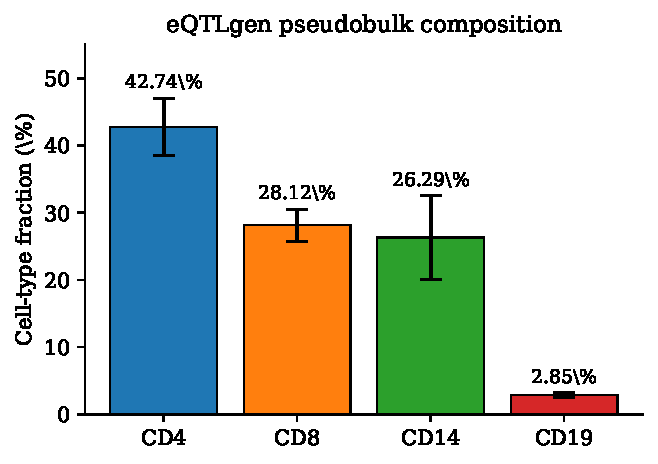
\includegraphics[width=0.6\textwidth]{figures/fig_eqtlgen_fractions.pdf}
\caption{Cell-type fractions used to generate pseudobulk samples from
eQTLgen scRNA-seq data. Means (SD): CD4 $42.74\%$ ($4.30$), CD8
$28.12\%$ ($2.40$), CD14 $26.29\%$ ($6.21$), CD19 $2.85\%$ ($0.36$).}
\label{fig:eqtlgen_fractions}
\end{figure}

\subsection{Sample-level cell fractions}

Accurate sample-level fractions are a prerequisite for every
deconvolution-based expression imputation step, so we began by
benchmarking fraction estimation alone against flow-cytometry ground
truth. We ran CIBERSORTx with the inbuilt LM22 signature (547 genes)
and with a custom signature derived from our training subjects
(1{,}589 genes), bMIND with the custom signature, and debCAM using the
1{,}247 cell-type-specific genes identified at $\mathrm{OVE.FC} = 10$.
Pearson correlation and RMSE against flow cytometry were computed per
test sample.

Pearson correlation with flow-measured fractions was highest for CD14,
followed by CD19, CD8 and CD4, regardless of method. CIBX-custom
performed less well than the other three approaches across all four
cell types, while CIBX-inbuilt and debCAM performed the best overall.
CD14 was systematically over-estimated and CD4 under-estimated by
every method, and bMIND and CIBX-custom occasionally returned fractions
of exactly zero for samples with clearly non-zero flow-measured
populations.

The gap between CIBX-custom and CIBX-inbuilt highlights the practical
importance of a well-trained signature: the inbuilt microarray-derived
matrix out-performed one built from our own RNA-seq, likely because
microarray signatures capture a more compact set of highly
discriminative genes. We therefore recommend CIBX-inbuilt and debCAM
as the default choices for fraction estimation from mixed-cell
RNA-seq, and carry the flow-measured fractions forward into the bMIND
and swCAM expression imputation so that any method that can use true
fractions gets the benefit of them.

\subsection{Accuracy of imputed sample-level cell-type expression}

Fraction accuracy is a means to an end; the quantity that matters for
downstream analyses is sample-level cell-type expression. Having
fixed the best fraction estimator for each method, we next turned to
the central question of this paper: how accurately can each approach
recover sample-level cell-type expression in held-out test subjects?
We compared CIBERSORTx (inbuilt and custom), bMIND with flow
fractions, swCAM with flow fractions, and multi-response LASSO and
ridge, with imputed expression evaluated against observed sorted-cell
data in the CLUSTER test subjects. The
methods differ markedly in how many genes they impute:
CIBERSORTx returned $5{,}779$--$11{,}794$ genes depending on cell
type, while every other method imputed all or almost all $18{,}871$
retained genes. Per-subject correlations between observed and imputed
expression were uniformly high (median $r > 0.85$) for every method,
with LASSO and ridge showing slightly higher correlations and slightly
lower log-RMSE than the deconvolution-based methods. However, baseline
correlations between observed expression in different subjects in the
same cell type were also high, which reflects that cell type rather
than subject explains most expression variance and limits the
discriminative power of this sample-level metric.

We therefore moved to a more informative measure: per-gene
correlation across test subjects. Under this view the picture is
coarser and more telling. Correlation per gene varied substantially
within every method; LASSO and ridge had slightly lower median log-RMSE
than other approaches, and swCAM performed notably worse for CD8, CD14
and CD19. To control for the fact that different methods impute
different gene sets, we repeated the analysis restricted to the
genes predicted by every method. As shown in
Figure~\ref{fig:common_genes}, these common sets contained
$3{,}837$ genes for CD4, $6{,}274$ for CD8, $5{,}185$ for CD14 and
$2{,}689$ for CD19. On the common sets the ordering of methods was
unchanged. Together, these analyses establish that correlation and
RMSE distinguish methods only weakly and point us toward a
task-oriented metric.

\begin{figure}[H]
\centering
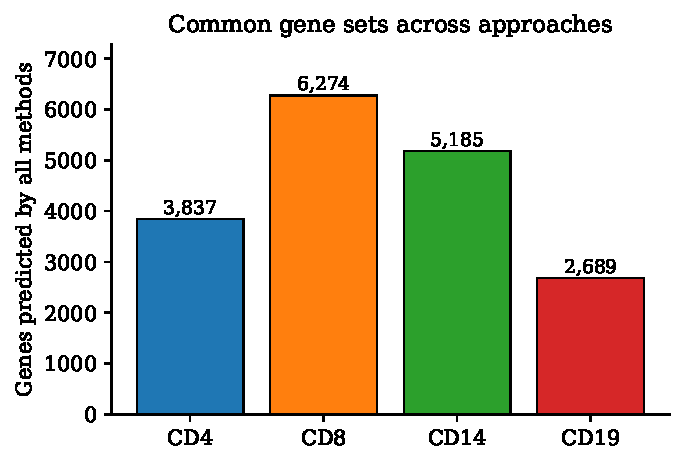
\includegraphics[width=0.6\textwidth]{figures/fig_common_genes.pdf}
\caption{Number of genes predicted by every method, used for the
common-gene sensitivity analysis: CD4 $3{,}837$; CD8 $6{,}274$; CD14
$5{,}185$; CD19 $2{,}689$.}
\label{fig:common_genes}
\end{figure}

\subsection{Differential-gene-expression recovery}

The correlation and RMSE analyses above rank methods weakly and offer
no direct read-out of downstream utility, so we next asked whether an
analyst running a routine differential-expression test on imputed data
would reach the same biological conclusions as on observed data.
Correlation and RMSE measure aggregate agreement between observed and
imputed expression but do not answer this question directly. We therefore defined a
differential-gene-expression recovery metric: for each simulated
phenotype we ran limma~\citep{ritchie2015limma} in parallel on observed
and imputed expression, fixed the observed FDR at $0.05$, varied the
imputed FDR from $0$ to $1$ in steps of $0.05$, and computed a receiver
operating characteristic AUC over the ten simulated phenotypes per
cell type.

In the CLUSTER cohort, LASSO and ridge regression achieved higher
median AUC than CIBERSORTx (inbuilt and custom), bMIND and swCAM in
every one of the four evaluated scenarios: a dichotomous phenotype, a
dichotomous phenotype with sex as a covariate, a continuous phenotype,
and a continuous phenotype with sex. Restricting the evaluation to the
common gene sets (CD4 $3{,}837$, CD8 $6{,}274$, CD14 $5{,}185$, CD19
$2{,}689$) preserved the ordering of methods. A detailed look at the
dichotomous scenario showed that LASSO and ridge achieved higher
sensitivity than CIBERSORTx, bMIND and swCAM, at the cost of lower
specificity: they call more genes significant in the imputed data,
including more of the genes that were significant in the observed
data. These results establish that penalised regression wins on the
task that motivates imputation in the first place---deciding which
genes respond to a phenotype---rather than on the aggregate agreement
metrics that have dominated the deconvolution literature to date.

Effect sizes tell a complementary story. In all methods, imputed
$\log_{2}$ fold changes were attenuated relative to those estimated
from observed data, with average slopes of $0.60$--$0.70$ in
CIBX-inbuilt, $0.64$--$0.76$ in CIBX-custom, $0.66$--$0.85$ in bMIND,
$0.55$--$0.90$ in swCAM, $0.69$--$0.76$ in LASSO, and $0.68$--$0.76$ in
ridge (Figure~\ref{fig:slopes}). LASSO and ridge showed the narrowest,
most consistent slope ranges across cell types, while swCAM had the
widest spread. No method recovered fold changes at face value, which
sets a hard ceiling on the claims that can be made from imputed data:
detection and direction of differential expression are supported;
unbiased magnitude is not.

\begin{figure}[H]
\centering
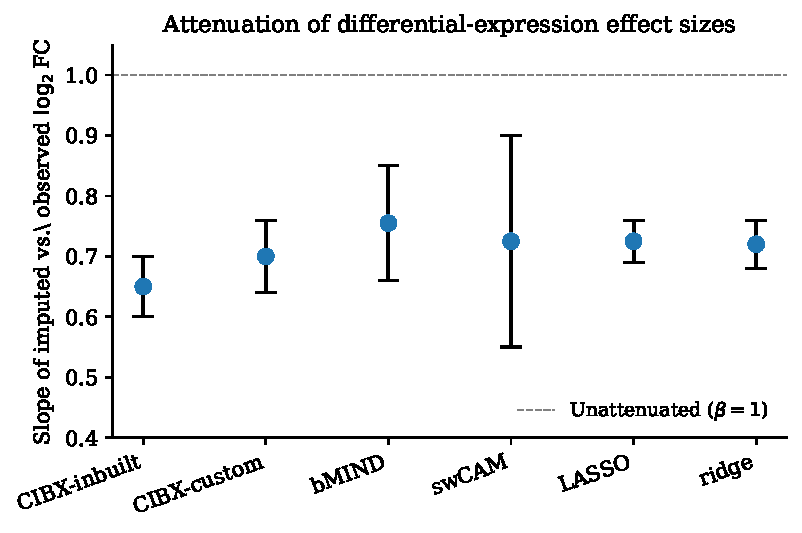
\includegraphics[width=0.75\textwidth]{figures/fig_slopes.pdf}
\caption{Attenuation of imputed $\log_{2}$ fold changes across methods.
Ranges across the four sorted cell types are shown as error bars around
the midpoint for each method. All methods shrink fold changes relative
to the unattenuated ideal ($\beta = 1$, dashed).}
\label{fig:slopes}
\end{figure}

The pseudobulk experiments let us probe how this picture changes with
training size. Across all three pseudobulk scenarios (raw counts with
condition as the DGE covariate, raw counts with batch and condition
covariates, and Combat-seq-adjusted counts with condition), AUC
increased monotonically with training size from 20 to 80 subjects
for every method, and LASSO and ridge consistently dominated
CIBERSORTx, bMIND and swCAM for CD4, CD8, CD14 and CD19. CIBERSORTx
with the inbuilt matrix imputed fewer than 60 genes for
CD19/Combat-seq, producing a very noisy AUC estimate in that single
cell. The dominance of penalised regression therefore holds under
batch correction as a covariate, under Combat-seq pre-correction, and
across a realistic stimulus-response contrast (C.~albicans at 3~h
versus untreated), reinforcing the CLUSTER finding.

\subsection{Computational performance}

Any practical recommendation must weigh accuracy against the resources
each method demands, especially as training-set sizes grow. We
therefore measured CPU time and peak memory for every method on both
CLUSTER and pseudobulk data under identical hardware conditions, and
report costs relative to CIBERSORTx as the reference
(Figure~\ref{fig:compute}). CPU time increased approximately
exponentially with training sample size for all methods, while peak
memory remained roughly constant. Relative to CIBERSORTx, which was
consistently the fastest method, bMIND was $2.7\times$ slower, swCAM
was $385\times$ slower, LASSO was up to $192.3\times$ slower and ridge
up to $658.1\times$ slower. Memory usage told a different story: bMIND
and swCAM needed only $33\%$ and $54\%$ of CIBERSORTx memory, whereas
LASSO required up to $3\times$ and ridge up to $11\times$ more than
CIBERSORTx. Penalised regression therefore trades memory and CPU for
accuracy, and the trade-off is well defined: on a cohort of 80
training subjects, a full LASSO run is comfortably tractable on a
workstation, whereas ridge becomes noticeably more expensive because
it retains non-zero coefficients for every PBMC predictor.

\begin{figure}[H]
\centering
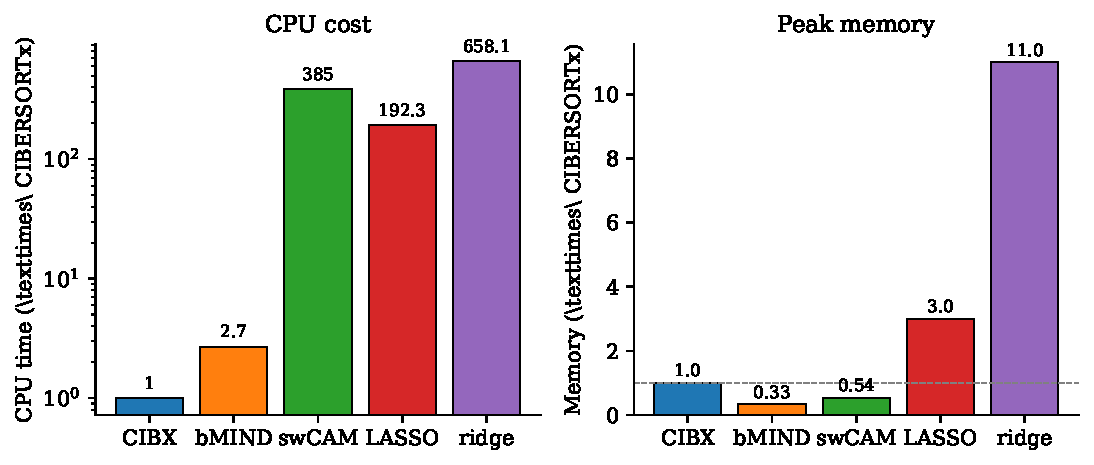
\includegraphics[width=0.9\textwidth]{figures/fig_compute.pdf}
\caption{Computational cost relative to CIBERSORTx. Left: CPU time on a
logarithmic scale; bMIND is $2.7\times$ slower, swCAM $385\times$,
LASSO $192.3\times$, ridge $658.1\times$. Right: peak memory; bMIND
uses $33\%$ and swCAM $54\%$ of CIBERSORTx memory, while LASSO and
ridge require up to $3\times$ and $11\times$, respectively.}
\label{fig:compute}
\end{figure}

\subsection{Summary tables}

\begin{table}[H]
\centering
\caption{Study design and sample counts by cell type and split.}
\label{tab:cohort}
\begin{tabular}{lcc}
\toprule
Cohort element & Training ($N$) & Test ($N$) \\
\midrule
PBMC (CLUSTER) & 80 & 78 \\
Sorted CD4 & 80 & 71 \\
Sorted CD8 & 80 & 65 \\
Sorted CD14 & 80 & 52 \\
Sorted CD19 & 80 & 57 \\
\midrule
eQTLgen pseudobulk (per dataset) & 20--80 & 80 \\
\bottomrule
\end{tabular}
\end{table}

\begin{table}[H]
\centering
\caption{Signature-gene counts by method.}
\label{tab:signatures}
\begin{tabular}{lcl}
\toprule
Signature set & No.\ genes & Source \\
\midrule
LM22 (CIBERSORTx inbuilt) & 547 & microarray, 22 leukocyte subsets \\
CIBX custom & 1{,}589 & 80 CLUSTER training subjects \\
debCAM OVE.FC=10 & 1{,}247 & 80 CLUSTER training subjects \\
\bottomrule
\end{tabular}
\end{table}

\begin{table}[H]
\centering
\caption{Slope of imputed vs.\ observed $\log_{2}$ fold changes (range across the four cell types).}
\label{tab:slopes}
\begin{tabular}{lc}
\toprule
Method & Slope range \\
\midrule
CIBX-inbuilt & 0.60--0.70 \\
CIBX-custom & 0.64--0.76 \\
bMIND & 0.66--0.85 \\
swCAM & 0.55--0.90 \\
LASSO & 0.69--0.76 \\
ridge & 0.68--0.76 \\
\bottomrule
\end{tabular}
\end{table}

\begin{table}[H]
\centering
\caption{Computational cost relative to CIBERSORTx.}
\label{tab:compute}
\begin{tabular}{lcc}
\toprule
Method & CPU time ($\times$ CIBERSORTx) & Memory ($\times$ CIBERSORTx) \\
\midrule
bMIND & 2.7 & 0.33 \\
swCAM & 385 & 0.54 \\
LASSO & 192.3 & 3 \\
ridge & 658.1 & 11 \\
\bottomrule
\end{tabular}
\end{table}

\begin{table}[H]
\centering
\caption{Multi-response LASSO/ridge gene-chunk counts (size ranges in parentheses).}
\label{tab:chunks}
\begin{tabular}{llcc}
\toprule
Dataset & Cell type & No.\ chunks & Size range \\
\midrule
CLUSTER & CD4 & 74 & 49--481 \\
CLUSTER & CD8 & 71 & 71--493 \\
CLUSTER & CD14 & 76 & 76--496 \\
CLUSTER & CD19 & 83 & 41--486 \\
Pseudobulk (24 datasets) & CD4 & 1{,}358 & 4--500 \\
Pseudobulk (24 datasets) & CD8 & 1{,}306 & 8--498 \\
Pseudobulk (24 datasets) & CD14 & 1{,}533 & 3--499 \\
Pseudobulk (24 datasets) & CD19 & 1{,}180 & 2--497 \\
\bottomrule
\end{tabular}
\end{table}

\section{Discussion}

Across a real paired cohort and 24 simulated pseudobulk datasets,
multi-response penalised regression consistently outperformed three
domain-specific deconvolution methods at the task that matters for
downstream biological analysis: recovering differential gene
expression signals that are present in observed sorted-cell data.
LASSO and ridge dominated CIBERSORTx (inbuilt and custom), bMIND and
swCAM on DGE-recovery AUC across every CLUSTER scenario (dichotomous
and continuous phenotypes, with and without sex adjustment) and across
every pseudobulk scenario (raw counts with or without batch
adjustment, and Combat-seq-corrected counts). The effect was robust to
restriction to common gene sets and persisted across training sizes
from 20 to 80 subjects. These findings establish penalised regression
as a strong default baseline for sample-level cell-type expression
imputation whenever paired PBMC and sorted-cell training data are
available.

The fraction-estimation comparison offers a subsidiary but practically
useful conclusion. CD4 fractions were the hardest to estimate for
every method, most likely because CD4 shares signature genes with CD8
and the number of truly CD4-specific markers is small. CIBERSORTx
with its inbuilt LM22 signature was the most accurate method for CD8,
while debCAM was the most accurate for CD4, but both clearly
out-performed CIBERSORTx with a custom signature and bMIND, which both
produced a number of implausible zero fractions in samples with
non-zero flow-measured populations. The broader lesson is that the
quality of the signature matrix matters more than the choice of
deconvolution algorithm; a well-validated signature derived from
matched-platform reference data will reliably beat one assembled ad
hoc from the data at hand.

The most interesting methodological result concerns the choice of
performance metric. Correlation per subject was high ($\mathrm{median}\
r > 0.85$) for every method, but the between-subject baseline
correlation was nearly as high, so the per-subject metric is dominated
by the fact that cell type explains most expression variance and says
little about how well individual-level imputation is working. Per-gene
correlation is more discriminative but still only a proxy for
analytical utility. The DGE-recovery AUC we introduced here maps a
concrete downstream analyst workflow to a single scalar, and it is in
this metric that the differences between methods become
unambiguous. We expect the DGE-recovery formulation to generalise to
any deconvolution benchmark where the downstream task is differential
expression, and to serve as a useful complement to the correlation and
RMSE measures that dominate the current
literature~\citep{avilacobos2020benchmarking}.

Why should a cross-domain machine-learning method outperform methods
explicitly designed for deconvolution? Two reasons emerge from our
analysis. First, deconvolution is a two-step inverse problem: an
estimate of cell fractions is used to solve for cell-type expression,
compounding the error at each step. Even bMIND and swCAM, which we
supplied with flow-measured fractions, did not match LASSO or ridge on
DGE recovery, suggesting that the error is not solely in the fraction
estimate. Second, LASSO and ridge are one-step: they learn the
PBMC-to-sorted map directly from paired training data, and multi-response
grouping lets them share regression coefficients across correlated
target genes, borrowing statistical strength exactly where the deconvolution
formulation assumes genes are independent. The cost of this statistical
sharing is computational: LASSO and ridge require up to $192.3\times$
and $658.1\times$ more CPU and $3\times$ and $11\times$ more memory
than CIBERSORTx respectively, and all penalised-regression estimates
still attenuate $\log_{2}$ fold changes to slopes of roughly
$0.68$--$0.76$. DGE analysis using imputed expression therefore supports
detection and direction of differential expression but not unbiased
effect-size estimation.

Several limitations temper these conclusions. The single most
important is that penalised regression requires paired PBMC and
sorted-cell training data, while deconvolution-based methods need only
a signature matrix or external fractions; in cohorts where no training
set exists, CIBERSORTx and debCAM remain the only viable options.
Second, we compared only four cell types---CD4, CD8, CD14 and
CD19---and a single mixed tissue (PBMC); rarer populations, or tissues
with more heterogeneous composition, may pose a different trade-off
between methods. Third, we have not optimised LASSO or ridge beyond
the default five-fold cross-validation choice of $\lambda$: better
gene-chunking strategies, group LASSO penalties, or deep-learning
alternatives could close the computational gap with CIBERSORTx while
preserving the accuracy advantage. Fourth, all methods systematically
attenuate fold-change magnitudes, which is a property of shrinkage
estimators and not a bug to be fixed, but which must be accounted for
when interpreting imputed-data effect sizes. Finally, our pseudobulk
simulation relies on the eQTLgen cell-type annotations and the
Jaakkola--Elo sampling scheme; departures from these assumptions could
shift the measured ordering of methods.

Taken together, the limitations above suggest that penalised
regression is not a universal solution but a strong baseline in a
well-defined regime. Looking forward, the clearest direction is to
expand the paired-data paradigm. Larger training cohorts, richer sets of sorted cell types,
and explicit modelling of technical batch effects within the
penalised-regression framework should all improve recovery without
changing the basic recipe. More sophisticated gene-grouping strategies
based on biological networks rather than expression-correlation
clusters could further reduce variance. Deep-learning encoders that
map PBMC expression directly to cell-type expression are an obvious
next step; they share the paired-training requirement of LASSO/ridge
but may exploit non-linear structure that the penalised linear model
misses. Across all of these directions, the task-oriented
DGE-recovery metric introduced here should serve as a common
yardstick: a method that looks good on correlation but loses on DGE
recovery is not, in the end, useful to the analyst who wants to know
which genes changed. Our broader recommendation is that cross-domain
machine-learning models should be the default baseline for
cell-type-specific expression imputation whenever paired training data
are available, and that domain-specific methods should be reserved
for the regime in which such data do not exist.

\bibliographystyle{plainnat}
\bibliography{references}

\end{document}
